\chapter{Introduzione}
Che cosa sono l'analisi e la Progettazione
\begin{itemize}
    \item Analisi - Enfatizza un'investigazione di un problema e dei suoi
    requisiti, anzichè di una soluzione
    \item La progettazione enfatizza una soluzione concettuale che soddisfa i requisiti
    del problema
\end{itemize}
Fare la cosa giusta (analisi) e fare la cosa bene (progettazione)
\section{Analisi e Progettazione orientata agli oggetti}
L'analisi orientata agli oggetti enfatizza sull'identificazione dei concetti o
degli oggetti, nel dominio del problema.
\\ La progettazione orentata agli oggetti enfatizza sulla definizione di oggetti
software che collaborano per soddisfare i requisiti.
\paragraph*{Esempio} Oggetti - Aereo, Volo, Pilota ognuno con i propri attributi
(tipo basi di dati).
Analisi e progettazione hanno obiettivi diversi che venogno perseguiti in modi diversi,
sono comunque attività sinergiche.
\\ L'OO (Object Oriented) enfatizza la rappresentazione di oggetti
\paragraph*{Definizione dei casi d'uso}
I casi d'uso sono delle store scritte relative al mondo in cui il sistema
viene utilizzato.
\paragraph*{Definizione di un modello di dominio}
Un modello di dominio mostra i concetti o gli oggetti significativi del dominio,
con i relativi attributi e associazioni.
\begin{center}
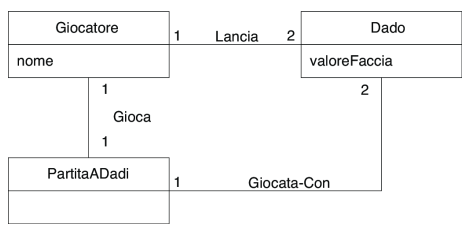
\includegraphics[width=100mm, scale=0.5]{modello_di_dominio_es.png}
\end{center}
\paragraph*{Definizione dei diagrammi di interazione}
Un diagramma di interazione mostra le collaborazioni tra oggetti software.
\begin{center}
    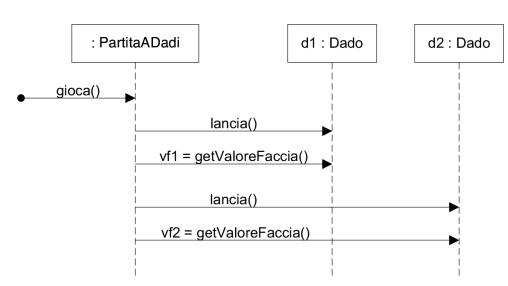
\includegraphics[width=100mm, scale=0.5]{diagramma_di_interazione_es.png}
\end{center}
\paragraph*{Definizioni dei diagramma delle classi di progetto}
Un diagramma delle classi di progetto mostra una vista statica delle definizioni
delle classi software, con i loro attributi e metodi.
\begin{center}
    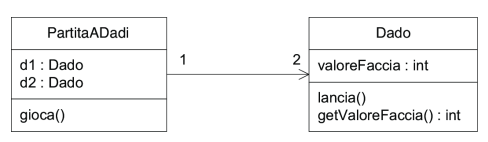
\includegraphics[width=100mm, scale=0.5]{diagramma_delle_classi_di_progetto.png}
\end{center}
Lo scopo di tutti questi diagrammi è facilitare la progettazione e il passaggio
da idea a codice.
\section{Che cosa è UML}
Unified Modelling Language (UML) è un linguaggio visuale di modellazione
dei sistemi e non solo.
Rappresenta una collezione di best practice di ingegneria, dimostratesi vincenti
nella modellazione di sistemi vasti e complessi. Dato che è lo standard de facto
favorisce la divulgazione di informazioni nella comunotà di ingegneri del software.
\\ \textbf{UML NON è una metodologia}
\begin{itemize}
    \item UML è un linguaggio visuale
    \item UP (Unified Process) è una metodologia
\end{itemize}
UML modella i sistemi come insiemi di oggetti che collaborano tra loro
\begin{itemize}
    \item Struttura Statica \begin{itemize}
        \item Quali tipo di oggetti sono necessari
        \item Come sono tra loro correlati
    \end{itemize}
    \item Struttura Dinamica \begin{itemize}
        \item Ciclo di vita di questi oggetti
        \item Come collaborano per fornire la funzionalità richieste
    \end{itemize}
\end{itemize}
\subsection{Tre modi per applicare UML}
\begin{itemize}
    \item UML come abbozzo
    \item UML come progetto
    \item UML come linguaggio di programmazione
\end{itemize}
\paragraph*{UML come Abbozzo} Diagrammi informali e incompleti (spesso abbozzati a mano)
che vengono creati per esplorare parti difficili dello spazio del problema o 
della soluzione, sfruttando l'espressività dei linguaggi visuali.
\paragraph*{UML come Progetto} Diagrammi di progetto relativamente dettagliati,
utilizzati per il reverse engineering, per la documentazione e per la comunicazione,
utilizzati quindi per visualizzare e comprendere meglio il codice esistente mediante
diagrammi UML.
\paragraph*{UML come linguaggio di programmazione} In questo caso il codice
viene generato direttamente e automaticamente da UML (approccio ancora in fase
di sviluppo).
\textbf{La modellazione agile enfatizza l'uso di UML come abbozzo}
\paragraph*{Due punti di vista per applicare UML}
\begin{itemize}
    \item Punto di vista concettuale - I diagrammi descrivono oggetti del mondo reale
    o in un dominio di interesse
    \item Punto di vista software - I diagrammi descrivono atrsazioni o componenti
    software
\end{itemize}
Entrambi usano la stessa notazione UML.
\subsection*{Il significato di classe nei diversi punti di vista}
Nell'UML grezzo, i rettangoli illustrati sono chiamati classi, questo termine
racchiude una varietà di casi: oggetti fisici, concetti astratti, elementi software, ecc.
\\ Il significato varia in base al diagramma di utilizzo, per fare chiarezza:
\begin{itemize}
    \item Classe concettuale - Oggetto o concetto del mondo reale - Significato
    attribuito nel \textbf{Modello di Dominio di UP}
    \item Classe software - Classe intesa come componente software (es. classe Java)
    - Significato attribuito nel \textbf{Modello di Progetto di UP}
\end{itemize}
\subsection{Vantaggi della mdoellazione visuale}
Disegnare o leggere UML implica che si sta lavorando in modo visuale e il nostro
cervello è più rapido a comprendere simboli, unità e relazioni rappresentati
con una notazione grafica.

\chapter{Processi per lo sviluppo del software}
Un processo per lo sviluppo del software (o processo software) definisce un approccio disciplinato
per la costruzione, il rilascio e la manutenzione del software.
\\ Definisce chi fa che cosa, quando e come per raggiungere un certo obiettivo.
\begin{itemize}
    \item Cosa - Sono le attività
    \item Chi - Sono i ruoli
    \item Come - Sono le metodologie
    \item Quando - Riguarda l'organizzazione temporale delle attività
\end{itemize}
\section{Che cos'è UP}
Un processo per lo sviluppo software descrive un approccio alla costruzione,
al rilascio ed eventualmente alla manutenzione del software. \textbf{Unified Process (UP)}
 è un processo iterativo diffuso per lo sviluppo del software per la costruzione di sistemi
 orientati ad oggetti.
 \\ UP è molto flessibile e aperto e incoraggia l'utilizzo di pratiche
 tratte da altri metodi iterativi come Extreme Programming (XP), Scrum, ecc.
 \paragraph{Riassumendo}
 \begin{itemize}
    \item UP è un processo iterativo
    \item Le pratiche UP forniscono una struttura di esempio
    \item UP è flessibile cioè iterativo, incrementale ed evolutivo
    \item Pilotato dai casi d'uso (requisiti) e dai fattori di rischio
    \item Incentrato sull'architettura
 \end{itemize}
\section{Il processo a cascata}
Il processo a cascata è il più vecchio tra quelli utilizzati oggi (definito tra gli
anni 60-70). Definito così per il suo ciclo di vita a cascata (o sequenziale),
basato sullo svolgimento sequenziale delle diverse attività dello sviluppo del software.
\\ Richiede che i requisiti siano chiari sin dall'inizio e spesso non è così dato
che durante la proggettazione emergono altri requisiti da parte del cliente.
\paragraph{Perchè il processo a cascata è soggeto a frequenti fallimenti}
\'E stata rilevata un'alta percentuale di fallimenti di progetti che utilizzano questo processo
e ci sono diversi motivi legati a questo alto tasso di fallimenti.
\\ Il motivo principale è che il processo a cascata presuppone che i requisiti siano
prevedibili e stabili e che possano essere definiti all'inizio, ma ciò è falso.
\' E stato dimostrato che ogni progetto software subisce mediamente il 25\% di cambiamenti
nei requisiti. Addirittura altri studi hanno evidenziato tassi dal 35 fino al 50\%, per quanto
riguarda i progetti più grandi.
Nello sviluppo software il presupposto che i requisiti siano stabili e prevedibili nel tempo
è fondamentalmente sbagliato. Nei progetti software il cambiamento è piuttosto una
costante.
\section{Sviluppo iterativo ed evolutivo}
Lo sviluppo iterativo ed evolutivo è una pratica fondamentale in molti processi
software moderni come UP e Scrum. In questo approccio al ciclo di vita,
lo sviluppo è organizzato in una serie di mini progetti brevi di lunghezza fissa
chiamati \textbf{iterazioni}. Ad ogni fase c'è un raffinamento del progetto a seguito
di feedback, per questo viene chiamato \textbf{sviluppo iterativo e incrementale}
o anche \textbf{sviluppo iterativo ed evolutivo}.
\\ L'instabilità dei requisiti e del progetto tende a diminuire nel tempo, 
nelle iterazioni finali è difficile (ma non impossibile), che si verifichi un
cambiamento significativo dei requisiti.
\subsection{Vantaggi dello sviluppo iterativo}
\begin{itemize}
    \item Minor probablità di fallimento del progetto
    \item Miglior produttività
    \item Percentuali più basse di difetti
    \item Riduzione precoce anzichè tardiva dei rischi maggiori
    \item Progesso visibile fin dall'inizio
    \item Feedback preoce e conseguente coinvolgimento dell'utente e adattamento
    \item Gestione della complessità
\end{itemize}
\subsection{Feedback e adattamento}
Attività fondamentale per il successo, come si struttura? E da dove proviene?
\begin{itemize}
    \item Feedback proveniente dalle attività di sviluppo
    \item Feedback proveniente dai test e dagli sviluppatori che raffinano il progetto e i modelli
    \item Feedback circa l'avanzamento del tema nell'affrontare i requisiti, per raffinare le stime
    dei tempi e dei costi
    \item Feedback proveniente dal cliente e dal mercato
\end{itemize}
\subsection{Durata delle iterazioni e timeboxing}
Una buona pratica dello sviluppo iterativo è il timeboxing: le iterazioni
hanno una lunghezza fissata (Molti processi iterativi raccomandano una lunghezza da 
2 a 6 settimane).
\\ Passi piccoli, feedback rapido e adattamento sono le idee centrali dello
sviluppo iterativo.
La durata di un'iterazione, una volta fissata non può cambiare, quando viene fissata
viene detta \textbf{timeboxed}.
\paragraph*{Non permettere al pensiero a cascata di invadere un progetto iterativo}
\subsection{Sviluppo iterativo e flessibilità del codice e del progetto}
L'adozione dello sviluppo iterativo richiede che il softare venga realizzato in modo flessibile
affinchè l'impatto dei cambiamenti sia basso. Il codice orgente deve quindi essere facilmente
modificabile e comprensibile (per facilitarne la modifica).
\textbf{flessibile}
\section{Come eseguire l'analisi e progettazione in modo iterativo
ed evoluto}
Un'attività critica nello sviluppo iterativo è la pianificazione delle iterazioni,
non bisogna tentare di pianificare tutto il progetto in modo dettagliato fin dall'inizio.
I processi iterativi promuovono la pianificazione guidata dal rischio e guidata dal cliente.
\subsection{Non cambiare gli obiettivi dell'iterazione}
Durante un'iterazione non è possibile cambiare i requisiti, dato che sono stati
precedentemente fissati durante la pianificazione iterativa e poi bloccati.
Questo perchè così facendo il Team di sviluppo può lavorare al suo meglio.
\subsection{Iterazioni - Perchè sono la chiave per UP}
Le iterazioni sono la chaive per UP, dato che ogni iterazione è come un mini-progetto 
che include:
\begin{itemize}
    \item Pianificazione
    \item Analisi e progettazione
    \item Costruzione
    \item Integrazione e test
    \item Un rilascio
\end{itemize}
Si arriva al rilascio finale attraverso una sequenza di iterazioni.
Le iterazioni possono sovrapporsi e questo è importante, dato che consente lo
sviluppo parallelo e il lavoro flessibile in grandi squadre.
Ad ogni iterazione si svolge una parte del lavoro totale di ogni disciplina.
\paragraph*{Esempio} Si svolgono in parallelo sia modellazione, Progettazione
 e implementazione, chiaramente a intensità diverse in base all'iterazione (e quindi
 alla fase del progetto), per esempio il testing sarà maggiore dopo qualche iterazione, 
 dato che ci saranno più cose da testare.
 \\ Ogni iterazione genera una \textbf{release} che costituisce un insieme di manufatti
 previsti e approvati. Un incremento è la differenza tra una release e quella successiva.
 Costituisce un passo in avanti verso il rilascio finale del sistema, per questo UP si chiama
 iterativo e incrementale.
 \section{Le fasi di UP}
 \begin{itemize}
    \item identificazione - Avvio del progetto
    \item Elaborazione - Realizzazione del nucleo dell'architettura
    \item Costruzione - Realizzazione delle capacità operative iniziali
    \item Transizione - Completamento del prodotto
 \end{itemize}
\subsection{Fasi e dicipline (o flussi di lavoro)}
\begin{center}
    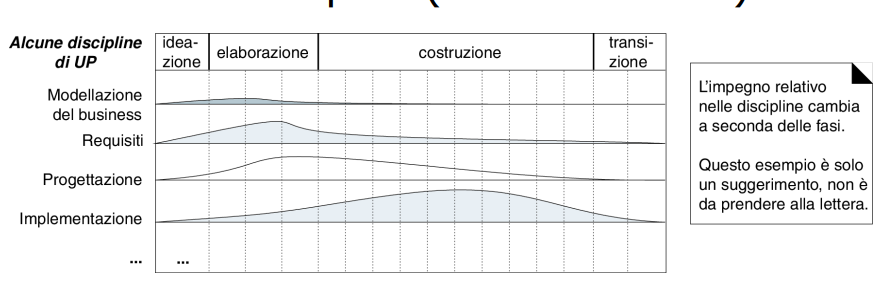
\includegraphics[width=100mm, scale=0.5]{FlussiDiLavoro.png}
\end{center}
Per ogni fase si considera:
\begin{itemize}
    \item L'attenzione in termini di flussi di lavoro
    \item L'obiettivo per la fase
    \item Il milestone alla fine della fase
\end{itemize}
Il processo con lo scenario di sviluppo di UP è nato per essere personalizzato,
per questo tra gli elaborati e le pratiche di UP, quasi tutto è opzionale.
\\ Alcune pratiche e principi sono fissi, come lo sviluppo iterativo e guidato dal rischio
e la verifica continua della qualità.
\\ Tutti gli elaborati (modelli, diagrammi, documenti) sono opzionali, con l'ovvia
esclusione del codice.
\\ La scelta delle pratiche degli elaborati UP per un progetto può essere scritta in un
breve documento chiamato scenario di sviluppo.
\begin{center}
    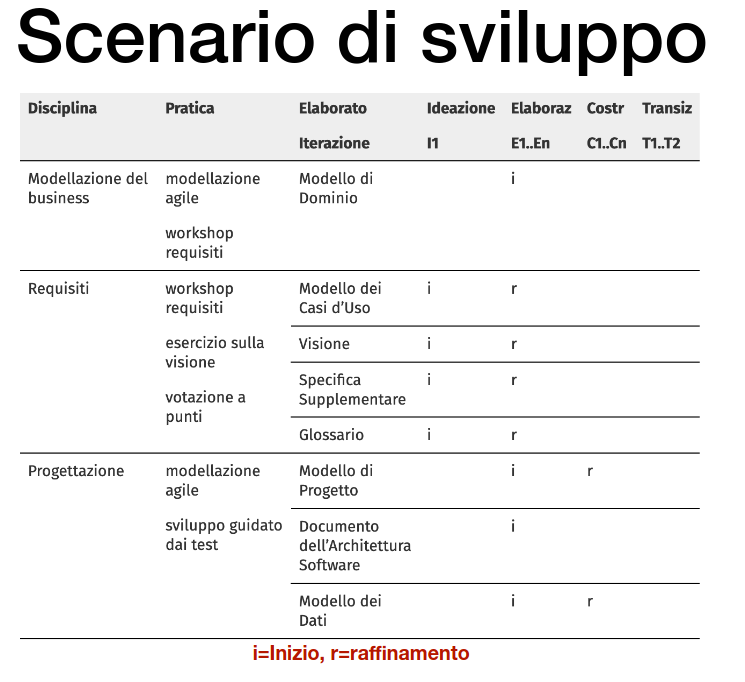
\includegraphics[width=100mm, scale=0.5]{esempio_scenario_sviluppo.png}
\end{center}
\paragraph*{Non si è capito lo sviluppo iterativo o UP se}
\begin{itemize}
    \item Si cerca di definire la maggior parte dei requisiti prima di iniziare
    la progettazione o l'implementazione
    \item Si pensa che i diagrammi UML e le attività di progettazione devono
    definire il progetto in dettaglio e che la programmazione è una mera traduzione
    di questi diagrammi
    \item Si ritiene che una durata adeguata per un'interazione sia tre mesi
    anzichè tre settimane
    \item Si prova a pianificare il progetto in dettaglio dall'inizio alla fine,
    in modo speculativo
\end{itemize}
Risulta quindi fondamentale ricordarsi che è un metodo per visualizzare il progetto,
per poter poi flessibilmente apportare modifiche, deve rimanere quindi agile.
Per dettagli vedere il Manifesto Agile.
\section{SCRUM}
Scrum è un metodo agile che consente di sviluppare e rilasciare prodotti software con il più alto valore
per i clienti ma nel più breve tempo possibile.
Scrum si occupa principalmente dell'organizzazione del lavoro e della gestione
di progetti.
\paragraph*{Terminologia}
\begin{itemize}
    \item Scrmum - Incontro giornaliero del Team SCRUM che esamina i progressi e definisce
    le priorità del lavoro da svolgere in quel giorno. Incontro breve faccia a faccia con tutto il team.
    \item ScrumMaster - Responsabile di assicurare che il processo di Scrum sia seguito e guida il team
    nell'uso efficace di Scrum. Responsabile dell'interfacciamento con il resto dell'azienda e di
    assicurare che il team non venga deviato da interferenze esterne
    \item Sprint - Un'iterazione di sviluppo. Le sprint sono solitamente di 2-4 settimane
    \item Velocity - Una stima di quanto lavoro rimanente un team può fare in un
    singolo sprint. Fondamentale per capire le prestazioni di una squadra e così
    migliorarle.
    \item Team di sviluppo - Un gruppo auto-organizzatore di sviluppatori di software,
    che non dovrebbe superare le 7 persone. Sono responsabili dello sviluppo del software e
    di altri documenti essenziali del progetto.
    \item Incremento potenzialmente rilasciabile - L'incremento software fornito da uno sprint
    \item Product Backlog - Questo è un elenco di elementi da fare (to do) che il team Scrum
    deve affrontare
    \item Product Owner - Può essere un cliente, ma potrebbe essere anceh un product manager
    in una società di software o un rappresentante di altri stakeholder. Identifica
    le caratteristiche o i requisiti del prodotto.
\end{itemize}

